\documentclass[11pt]{article}
% =========================================================================
% SHARED STYLE FILE for 11_Master_Projects reports
% Visual style follows 0_Thesis_Submission/24m0553_AK_Gaurav_Mtech_Report.pdf:
% serif body font, blue hyperlinked TOC/links, ruled section headings,
% IITB-style title page, formal academic report structure.
% =========================================================================

\usepackage[a4paper,margin=1in]{geometry}
\usepackage{xcolor}
\usepackage{graphicx}
\graphicspath{{../images/}}
\usepackage{amsmath,amssymb}
\usepackage{booktabs}
\usepackage{caption}
\usepackage{float}
\usepackage[hidelinks]{hyperref}
\usepackage{titlesec}
\usepackage{enumitem}
\usepackage{setspace}
\usepackage[T1]{fontenc}
\usepackage{lmodern}
\usepackage{microtype}

% Every \includegraphics call is automatically framed with a thin black
% border (matches the printed look of figures/photos/charts in the source
% reports). \oldincludegraphics is kept available for institutional
% logos/seals on title pages, which should remain unframed.
\let\oldincludegraphics\includegraphics
\setlength{\fboxsep}{1pt}
\setlength{\fboxrule}{0.6pt}
\renewcommand{\includegraphics}[2][]{\fbox{\oldincludegraphics[#1]{#2}}}

\definecolor{thesisblue}{RGB}{0,0,205}
\hypersetup{
  colorlinks=true,
  linkcolor=thesisblue,
  urlcolor=thesisblue,
  citecolor=thesisblue,
  filecolor=thesisblue
}

\onehalfspacing
\setlength{\parskip}{6pt}
\setlength{\parindent}{0pt}

\titleformat{\section}
  {\normalfont\Large\bfseries}{\thesection}{1em}{}
\titleformat{\subsection}
  {\normalfont\large\bfseries}{\thesubsection}{1em}{}
\titleformat{\subsubsection}
  {\normalfont\normalsize\bfseries}{\thesubsubsection}{1em}{}

\newcommand{\reportTitlePage}[7]{%
  % #1 = Report title
  % #2 = Course code & name (e.g. "CE 605: Applied Statistics")
  % #3 = Subtitle/topic line (e.g. "Project Report 2: Network Analysis")
  % #4 = Author block (can be multi-line with \\ for group projects)
  % #5 = Supervisor name(s)
  % #6 = Programme line (e.g. "M.Tech in Transportation Systems Engineering")
  % #7 = Month/Year
  \begin{titlepage}
    \centering
    \vspace*{0.5cm}
    {\large\bfseries #2}\par
    \vspace{0.3cm}
    {\Large\bfseries #3}\par
    \vspace{1.2cm}
    {\Huge\bfseries #1}\par
    \vspace{1.5cm}
    \oldincludegraphics[width=3.2cm]{../../assets/iitb_logo.png}\par
    \vspace{1.2cm}
    Submitted by:\par
    \vspace{0.2cm}
    {\bfseries #4}\par
    \vspace{0.8cm}
    Under the Supervision of\par
    \vspace{0.2cm}
    {\bfseries #5}\par
    \vspace{1.2cm}
    #6\par
    Department of Civil Engineering\par
    \textbf{Indian Institute of Technology Bombay}\par
    Mumbai -- 400076, India\par
    \vspace{0.3cm}
    #7\par
  \end{titlepage}
}

\newcommand{\reportAbstract}[1]{%
  \section*{Abstract}
  #1
  \vspace{0.5cm}
}

\usepackage{longtable}

\title{CE 773 Coursework Assignments: Geometric Design and Analysis of High-Speed Roadways}
\author{Abhijeet Kumar Gaurav}
\date{}

\begin{document}

\reportTitlePage
  {CE 773 Coursework Assignments: Geometric Design and Analysis of High-Speed Roadways}
  {CE 773: Geometric Design and Analysis of High-Speed Roadways}
  {Compiled Coursework Assignments 1--4}
  {Abhijeet Kumar Gaurav \\ Roll No.: 24M0553}
  {Prof. Avijit Maji}
  {M.Tech in Transportation Systems Engineering}
  {Spring 2025}

\pagenumbering{roman}

\reportAbstract{
This document compiles four coursework assignments submitted for CE 773: Geometric Design and
Analysis of High-Speed Roadways, at the Indian Institute of Technology Bombay. Assignment~1 reviews
the geometric design concepts applied in the Agra--Lucknow Expressway project. Assignment~2 estimates
the Average Daily Traffic (ADT) and 30th-hour design volume for a rural four-lane highway from 50 days
of hourly traffic-count data, and evaluates the Level of Service (LOS) over a 10-year design horizon to
assess whether a 4-to-6 lane capacity expansion is warranted. Assignment~3 develops the tangent
cross-section of a four-lane expressway located in the high-rainfall North-East region of India, based
on IRC design guidelines. Assignment~4 is a field-based geometric design and safety review of the H10
intersection on the IIT Bombay campus. Each assignment is reproduced here as submitted, organised as
one section per assignment, with the original questions, calculations, tables, and figures preserved.
Assignment~1 was a group submission completed jointly with Shivam Singh (Roll No.\ 24M0552), and
Assignment~4 was a group submission completed jointly with Karshan M.\ Kanjariya (24D0322), Irfan Ali
(24D0314), Menbere Aklilu (24D0315), and Fred Ssemwogerere (24D0326); this is noted explicitly in the
respective sections below. Assignments~2 and~3 were solo submissions.

\vspace{0.3cm}
\noindent\textbf{Keywords:} Highway Geometric Design; Traffic Volume Analysis; Level of Service;
Expressway Cross-Section; Intersection Safety Review; IRC Design Standards
}

\newpage
\tableofcontents
\newpage
\pagenumbering{arabic}

\section{Assignment 1: Case Study Review -- Agra--Lucknow Expressway}

\textbf{Group submission note:} This assignment was completed jointly with Shivam Singh (Roll No.\
24M0552), as recorded on the original submission. The content below reproduces the submitted group
report.

\textbf{Question.} Review any significant highway development project implemented in the last decade
and describe the different design concepts applied.

\subsection{Project Overview}
The Agra--Lucknow Expressway, a 302.22~km access-controlled, six-lane expressway in Uttar Pradesh, was
reviewed to evaluate its geometric design concepts and how it addresses challenges in transportation,
safety, and sustainability. The expressway was developed to tackle transportation issues in Uttar
Pradesh, reducing travel time from over 6 hours to approximately 3.5 hours between Agra and Lucknow,
addressing congestion and safety concerns on NH-19, and integrating districts including Kannauj,
Auraiya, and Unnao.

\begin{table}[H]
  \centering
  \caption{Agra--Lucknow Expressway: project overview.}
  \begin{tabular}{@{}ll@{}}
    \toprule
    \textbf{Feature} & \textbf{Details} \\
    \midrule
    Length & 302.22 km \\
    Lanes & 6 lanes, expandable to 8 lanes \\
    Construction period & January 2015 to November 2016 \\
    Completion time & 22 months \\
    Inauguration date & 21 November 2016 \\
    Travel time reduction & From 6 hours to approximately 3.5 hours \\
    Starting point & Agra Inner Ring Road \\
    Ending point & State Highway 40 in Lucknow \\
    Districts covered & Agra, Firozabad, Mainpuri, Etawah, Auraiya, Kannauj, \\
                       & Kanpur Nagar, Hardoi, Unnao, Lucknow \\
    \bottomrule
  \end{tabular}
\end{table}

\begin{table}[H]
  \centering
  \caption{Cost overview.}
  \begin{tabular}{@{}ll@{}}
    \toprule
    \textbf{Aspect} & \textbf{Details} \\
    \midrule
    Initial estimated cost & Rs.~15{,}000 crore \\
    Final completion cost & Rs.~13{,}200 crore \\
    Cost savings & Rs.~1{,}800 crore \\
    \bottomrule
  \end{tabular}
\end{table}

\begin{table}[H]
  \centering
  \caption{Major stakeholders.}
  \begin{tabular}{@{}ll@{}}
    \toprule
    \textbf{Stakeholder} & \textbf{Role} \\
    \midrule
    Government of Uttar Pradesh & Project financing and oversight \\
    UP Expressways Industrial Development & Project implementation and \\
    Authority (UPEIDA) & management \\
    Construction contractors & Various firms responsible for different \\
                             & sections of the expressway \\
    Local communities & Benefit from improved connectivity and \\
                       & economic opportunities \\
    \bottomrule
  \end{tabular}
\end{table}

\subsection{Design Concepts Applied}

\subsubsection{Greenfield Alignment Design}
The expressway was built to solve problems with the busy NH-19 road, which faced heavy traffic, delays,
and safety concerns. Expanding the old road would have needed much land in crowded areas, causing more
displacement and higher costs. The new expressway takes a shorter route around cities, allowing faster
and smoother travel; advanced technologies such as GIS and LiDAR were used in its planning.

\subsubsection{Complete Street Concepts}
The Agra--Lucknow Expressway does not incorporate complete street concepts to accommodate all users,
including pedestrians, cyclists, motorists, and transit vehicles. It is designed only for fast-moving
vehicles and does not have bike lanes or sidewalks for non-motorized users; it is focused on high-speed
travel rather than mixed-use transportation. However, side roads for local access allow residents to
reach their destinations.

\subsubsection{Median and Roadside Safety Design}
The expressway has wide medians (10--12~m) and crash barriers to help prevent head-on collisions and
reduce the severity of accidents. The landscaped medians also improve the aesthetic and environmental
character of the corridor, balancing safety with visual appeal.

\subsubsection{Context-Sensitive Solutions (CSS)}
The expressway aligns well with context-sensitive solutions by addressing the region's specific needs
while minimising environmental and social impact. The alignment was carefully planned to avoid urban
centres, reducing disruptions in densely populated areas. The project also integrates green
infrastructure, such as green belts along the expressway, noise barriers to reduce sound pollution, and
rainwater harvesting pits every 500~m to address water management.

\subsubsection{Performance-Based Design}
The expressway's performance-based design ensures safety and operational efficiency. Grade-separated
intersections remove level crossings, improving traffic flow and reducing delays; flyovers and
underpasses are placed at key crossroads, while trumpet and cloverleaf interchange designs enhance
connectivity and minimise conflict points. Intelligent Transport Systems (ITS), including surveillance
cameras, electronic call boxes, digital message boards, and incident detection systems, further enhance
safety and traffic management.

\subsubsection{Practical Design}
The expressway adopts a practical design approach, focusing on essential features to balance cost and
functionality: limited interchanges for access control, service roads for local traffic, rumble strips,
and reflective signage. This approach enabled the expressway to be completed within budget while
meeting high operational standards.

\textbf{Emergency airstrip integration.} A standout feature of the expressway is its 3.3~km-long
emergency airstrip near Unnao, designed to support disaster management and defense operations. Before
this project, India lacked infrastructure capable of handling emergency fighter-jet landings on
highways; the airstrip supports Indian Air Force (IAF) and disaster relief operations.

\subsubsection{Design Matrix Approach}
The design matrix approach was not explicitly applied during the planning and construction phases of
the expressway. While this method typically involves choosing between basic, modified, or complete
design standards based on project goals, the expressway adheres to high-speed geometric standards
suitable for its purpose without a formal design matrix.

\subsubsection{Safe System Approach}
The expressway prioritises safety with well-designed curves, wide medians, crash barriers, and a
120~km/h speed limit. ITS enhances safety through prompt incident detection and response; green
(solar) energy is used for all illumination; staggered service roads are provided on both sides of the
expressway except at major bridges and RoBs; and patrolling vehicles and GPS-based ambulance services
ensure rapid assistance within 4--11 minutes.

\subsubsection{Travel Time Reliability Approach}
The travel time reliability approach has improved consistency and predictability by eliminating traffic
signals, restricting access, and integrating real-time traffic monitoring, reducing travel time between
Agra and Lucknow to about 3.5 hours.

\subsubsection{Value Engineering}
The expressway successfully utilised value engineering to optimise costs without compromising quality.
Through efficient land acquisition, streamlined construction processes, and practical design practices,
the project achieved cost savings of Rs.~1,800 crore, reducing total expenditure from an initial
estimate of Rs.~15,000 crore to Rs.~13,200 crore.

\subsubsection{Designing of 3R Projects}
The Agra--Lucknow Expressway is a greenfield project built from scratch and does not fall under 3R
projects (Resurfacing, Restoration, Rehabilitation). Unlike 3R projects that upgrade existing
infrastructure, it is a new access-controlled highway designed for high-speed connectivity without links
to older roads.

\subsubsection{Performance-Based Practical Design (PBPD)}
The expressway is designed for good performance while keeping costs down. It starts with six lanes but
can be expanded to eight if needed, includes technology for traffic management, and incorporates green
spaces for sustainability -- a design focused on safety, usability, and budget that can adapt to future
needs.

\clearpage
\section{Assignment 2: ADT, 30th-Hour Design Volume, and LOS Forecast for a Rural Four-Lane Highway}

\textbf{Question 1.} In a rural median-divided four-lane highway development project, find the design
traffic volume. The hourly traffic volume (in PCU) for 50 days per calendar year for one direction is
provided in a spreadsheet keyed to the student's roll number. Estimate the ADT and the 30th-hour design
volume, showing calculations step by step.

\subsection{Given Data}
\begin{itemize}
  \item Rural, median-divided, four-lane highway.
  \item Hourly traffic volume (in PCU) for 50 days per calendar year, one direction.
\end{itemize}

\subsection{Step-by-Step Solution}

\textbf{(i) Estimation of ADT.} The Average Daily Traffic (ADT) is the total volume during a given
period (greater than one day, less than one year), divided by the number of days in that period. Here,
time period = 50 days; sum of daily traffic (for 50 days) = 1{,}638{,}192.
\[
\text{ADT} = \frac{1{,}638{,}192}{50} = 32{,}763.84 \text{ PCU/day/lane}
\]
\textit{Inference:} the average number of vehicles passing the section per day over the observed period
was approximately 32{,}763 PCU per day per lane.

\textbf{(ii) Estimation of 30th-hour design volume.}
\begin{itemize}
  \item \textit{Step 1.} Combine all traffic data for 50 days into one column, giving $50 \times 24 =
  1200$ hourly rows.
  \item \textit{Step 2.} Sort the 1200 values in descending order.
  \item \textit{Step 3.} Identify the 30th highest value -- the value exceeded 29 times.
\end{itemize}
\textbf{Result:} the 30th-hour design volume = \textbf{2157 PCU/hr/lane}.

Figure~\ref{fig:hourly-volume} shows the hourly-volume curve (hourly two-way traffic volume as a
percentage of ADT, plotted against the number of hours in one year with volume greater than that shown),
with the 30th and 100th highest-hour markers indicated. As noted on the original chart, this curve comes
out as a straight line because the dataset covers only 50 days rather than a full year, which affects
the design-volume consideration. Since there is no sizeable seasonal variation apparent in the data, the
30th highest volume is taken as 15\% of ADT.

\begin{figure}[H]
  \centering
  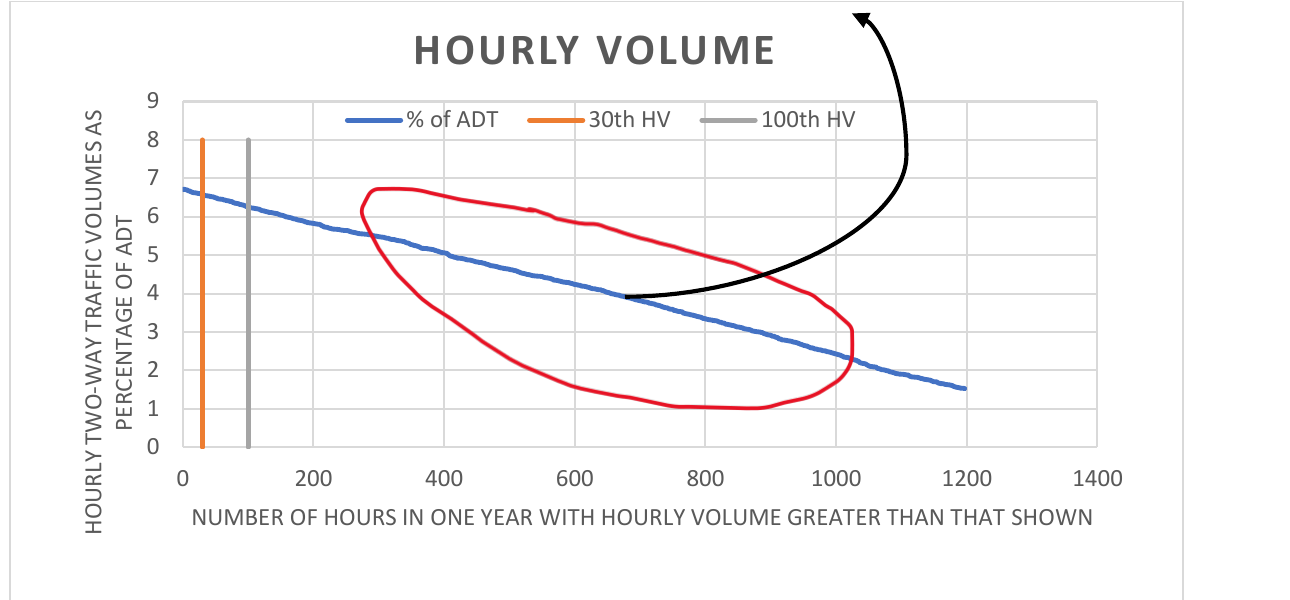
\includegraphics[width=0.85\textwidth]{fig_a2_hourly_volume_chart.png}
  \caption{Hourly two-way traffic volumes as a percentage of ADT, showing the 30th and 100th highest-hour
  markers (as plotted in the original submission).}
  \label{fig:hourly-volume}
\end{figure}

\textbf{Question 2.} The operating speed of the highway in Question~1 is 100~km/h. Using the estimated
design volume, review the design improvement required over the next 10 years. The expected LOS at any
point should not fall below ``C.'' Any improvement takes about 3 years for design, ROW acquisition, and
construction. Show the evaluation and decision-making process step by step.

\subsection{Given Data and Constraints}
\begin{itemize}
  \item Operating speed = 100 km/h; capacity for 4 lanes = 4540 PCU/hr per 2-lane carriageway; capacity
  for 6-lane divided highways = 6790 PCU/hr per 3-lane carriageway.
  \item Growth rate = 5\% (per IRC).
  \item Expected LOS at any point should not fall below ``C.''
  \item Design, ROW acquisition, and construction take about 3 years.
\end{itemize}

\subsection{Step 1: Analysis of the Present Scenario Using the 30th-Hour Design Volume}
Using the present design volume of 2157~PCU/hr/lane against a capacity of 4540~PCU/hr/lane, and
projecting forward at a 5\% annual growth rate using
\[
\text{Future Volume} = \text{Current Volume} \times (1+\text{Growth Rate})^{\text{Years}},
\]
the future volume after 10 years is $2157 \times (1.05)^{10} = 3513.53$ PCU/hr/lane.

\begin{table}[H]
  \centering
  \caption{4-lane divided highway: design volume, v/c ratio, and LOS over 10 years, based on the 30th-hour design volume.}
  \resizebox{\textwidth}{!}{%
  \begin{tabular}{@{}lrrrrrrrrrrr@{}}
    \toprule
    \textbf{Year} & Current & 1 & 2 & 3 & 4 & 5 & 6 & 7 & 8 & 9 & 10 \\
    \midrule
    Design volume & 2157 & 2264.85 & 2378.09 & 2497.00 & 2621.85 & 2752.94 & 2890.59 & 3035.12 & 3186.87 & 3346.21 & 3513.53 \\
    Capacity & 4540 & 4540 & 4540 & 4540 & 4540 & 4540 & 4540 & 4540 & 4540 & 4540 & 4540 \\
    v/c & 0.4751 & 0.4989 & 0.5238 & 0.5501 & 0.5775 & 0.6064 & 0.6367 & 0.6685 & 0.7020 & 0.7371 & 0.7739 \\
    LOS & C & C & D & D & D & D & D & E & E & E & E \\
    \bottomrule
  \end{tabular}%
  }
\end{table}

The 4-lane highway maintains LOS~C only until year~2, after which it drops to LOS~D and eventually
LOS~E. Since LOS begins dropping after the 1st year, using the 30th-hour design volume directly does not
leave enough time (3 years are required) to complete a capacity-improvement construction before the LOS
constraint is violated. The design volume therefore needs to be reconsidered.

\subsection{Step 2: Selecting a More Suitable Design Volume}
Per IRC guidance on Design Hourly Volume for rural four-lane highways, design typically assumes moderate
traffic growth over the next 10--20 years, and the 95th-percentile volume is sometimes used to account
for more extreme future traffic conditions. Analysing the frequency distribution of the one-lane traffic
volumes (Figure~\ref{fig:histogram}) shows that most traffic volumes (266, 270, 299, 294 hours in the
respective bins) fall in the lower ranges, between 500 and 2100 PCU, while the $(2100,2500]$ range has
the least volume (71 hours), indicating that high traffic volumes in this range are rare. The roadway
therefore experiences moderate traffic conditions, with infrequent occurrences of exceptionally high
volumes.

\begin{figure}[H]
  \centering
  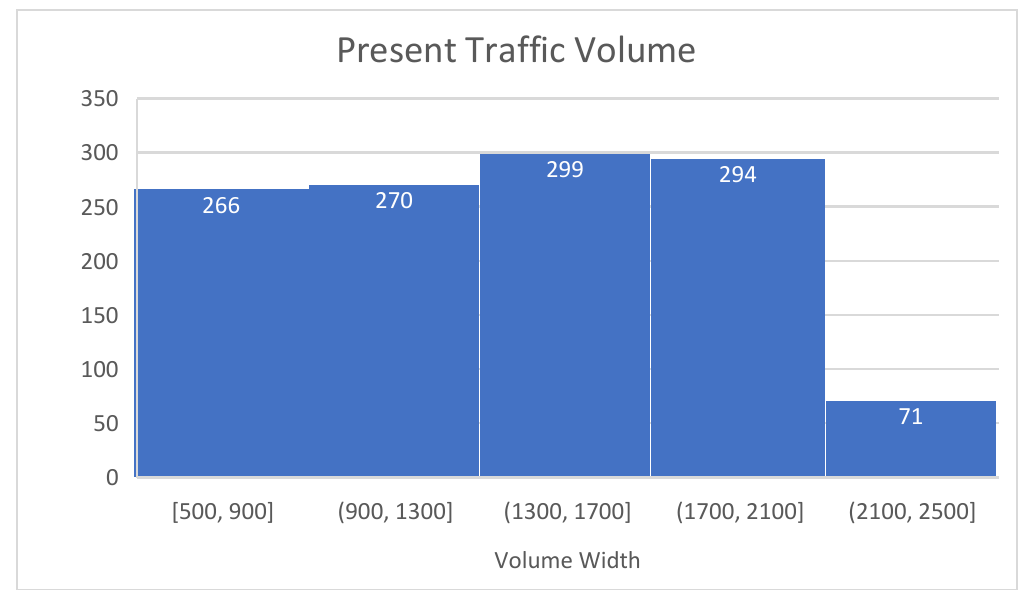
\includegraphics[width=0.7\textwidth]{fig_a2_present_traffic_histogram.png}
  \caption{Frequency distribution (histogram) of present hourly traffic volume, by volume-width bin (as plotted in the original submission).}
  \label{fig:histogram}
\end{figure}

\textbf{Conclusion:} the \textbf{85th-percentile volume} is adopted as the estimated design volume
instead of the 30th-hour value.

\subsection{Step 3: Calculation of the 85th-Percentile Volume}
To find the 85th percentile rank in a sorted (ascending) list of 1200 hourly values ($50$ days
$\times 24$ hours):
\[
\text{Percentile Rank} = 0.85 \times 1200 = 1020^{\text{th}} \text{ value}
\]

\begin{table}[H]
  \centering
  \caption{Percentile ranks and corresponding design volumes.}
  \begin{tabular}{@{}lrr@{}}
    \toprule
    \textbf{Percentile} & \textbf{Position (th)} & \textbf{Design volume (PCU/hr/2-lane)} \\
    \midrule
    97.5th percentile & 1164 & 2157 \\
    95th percentile   & 1140 & 2115 \\
    85th percentile   & 1020 & 1935 \\
    \bottomrule
  \end{tabular}
\end{table}

\subsection{Step 4: Traffic Growth and Lane-Configuration Decision}

\begin{table}[H]
  \centering
  \caption{Design volume, v/c ratio, and LOS over 10 years for the 4-lane and 6-lane divided configurations, based on the 85th-percentile volume.}
  \resizebox{\textwidth}{!}{%
  \begin{tabular}{@{}lrrrrrrrrrrr@{}}
    \toprule
    \textbf{Year} & 1 & 2 & 3 & 4 & 5 & 6 & 7 & 8 & 9 & 10 \\
    \midrule
    Design volume & 1935 & 2031.75 & 2133.34 & 2240.00 & 2352.00 & 2469.60 & 2593.09 & 2722.74 & 2858.88 & 3001.82 \\
    \addlinespace
    \multicolumn{11}{@{}l}{\textbf{4-lane divided}} \\
    Capacity & 4540 & 4540 & 4540 & 4540 & 4540 & 4540 & 4540 & 4540 & 4540 & 4540 \\
    v/c  & 0.4262 & 0.4475 & 0.4699 & 0.4934 & 0.5181 & 0.5440 & 0.5712 & 0.5997 & 0.6297 & 0.6612 \\
    LOS  & C & C & C & C & D & D & D & D & D & D \\
    \addlinespace
    \multicolumn{11}{@{}l}{\textbf{6-lane divided} (from year 4 onward)} \\
    Capacity & -- & -- & -- & 6790 & 6790 & 6790 & 6790 & 6790 & 6790 & 6790 \\
    v/c  & -- & -- & -- & 0.3300 & 0.3464 & 0.3637 & 0.3819 & 0.4010 & 0.4210 & 0.4421 \\
    LOS  & -- & -- & -- & C & C & C & C & C & C & C \\
    \bottomrule
  \end{tabular}%
  }
\end{table}

\textbf{Overall result.} The 6-lane configuration, introduced from year 4 with a capacity of 6790
PCU per hour per lane, keeps the v/c ratio well below the LOS-D threshold, stabilising between approximately
0.33 and 0.44 over the remaining years. By expanding from 4 to 6 lanes starting in the present year, the
road maintains LOS~C throughout the initial years and avoids the drop to LOS~D that would otherwise occur
around year~4--5 under the 4-lane configuration. \textbf{This justifies a 4-to-6 lane capacity expansion}
within the 10-year design horizon considered.

\clearpage
\section{Assignment 3: Tangent Cross-Section of a Four-Lane Expressway in North-East India}

\textbf{Question.} Develop the cross-section of a four-lane expressway for a tangent section. This
expressway is located in the open country of the north-east region of India, where the annual rainfall
is about 200~cm. Assume appropriate details from the relevant IRC code(s). Choose a suitable horizontal
and vertical scale to represent the cross-section on graph paper.

\subsection{Relevant Cross-Section Elements}
Figure~\ref{fig:cross-section-elements} reproduces the typical cross-section element taxonomy used to
identify which elements are relevant to a tangent-section design. Of the full set of cross-section
elements (pavement surface characteristics, cross-slope/camber, carriageway width, median/traffic
separators, kerbs, shoulders, edge strips, road margins, and so on), only those highlighted in the
original submission -- width of carriageway, shoulders, median, road margins, roadway width, and
right-of-way -- were needed to develop this design.

\begin{figure}[H]
  \centering
  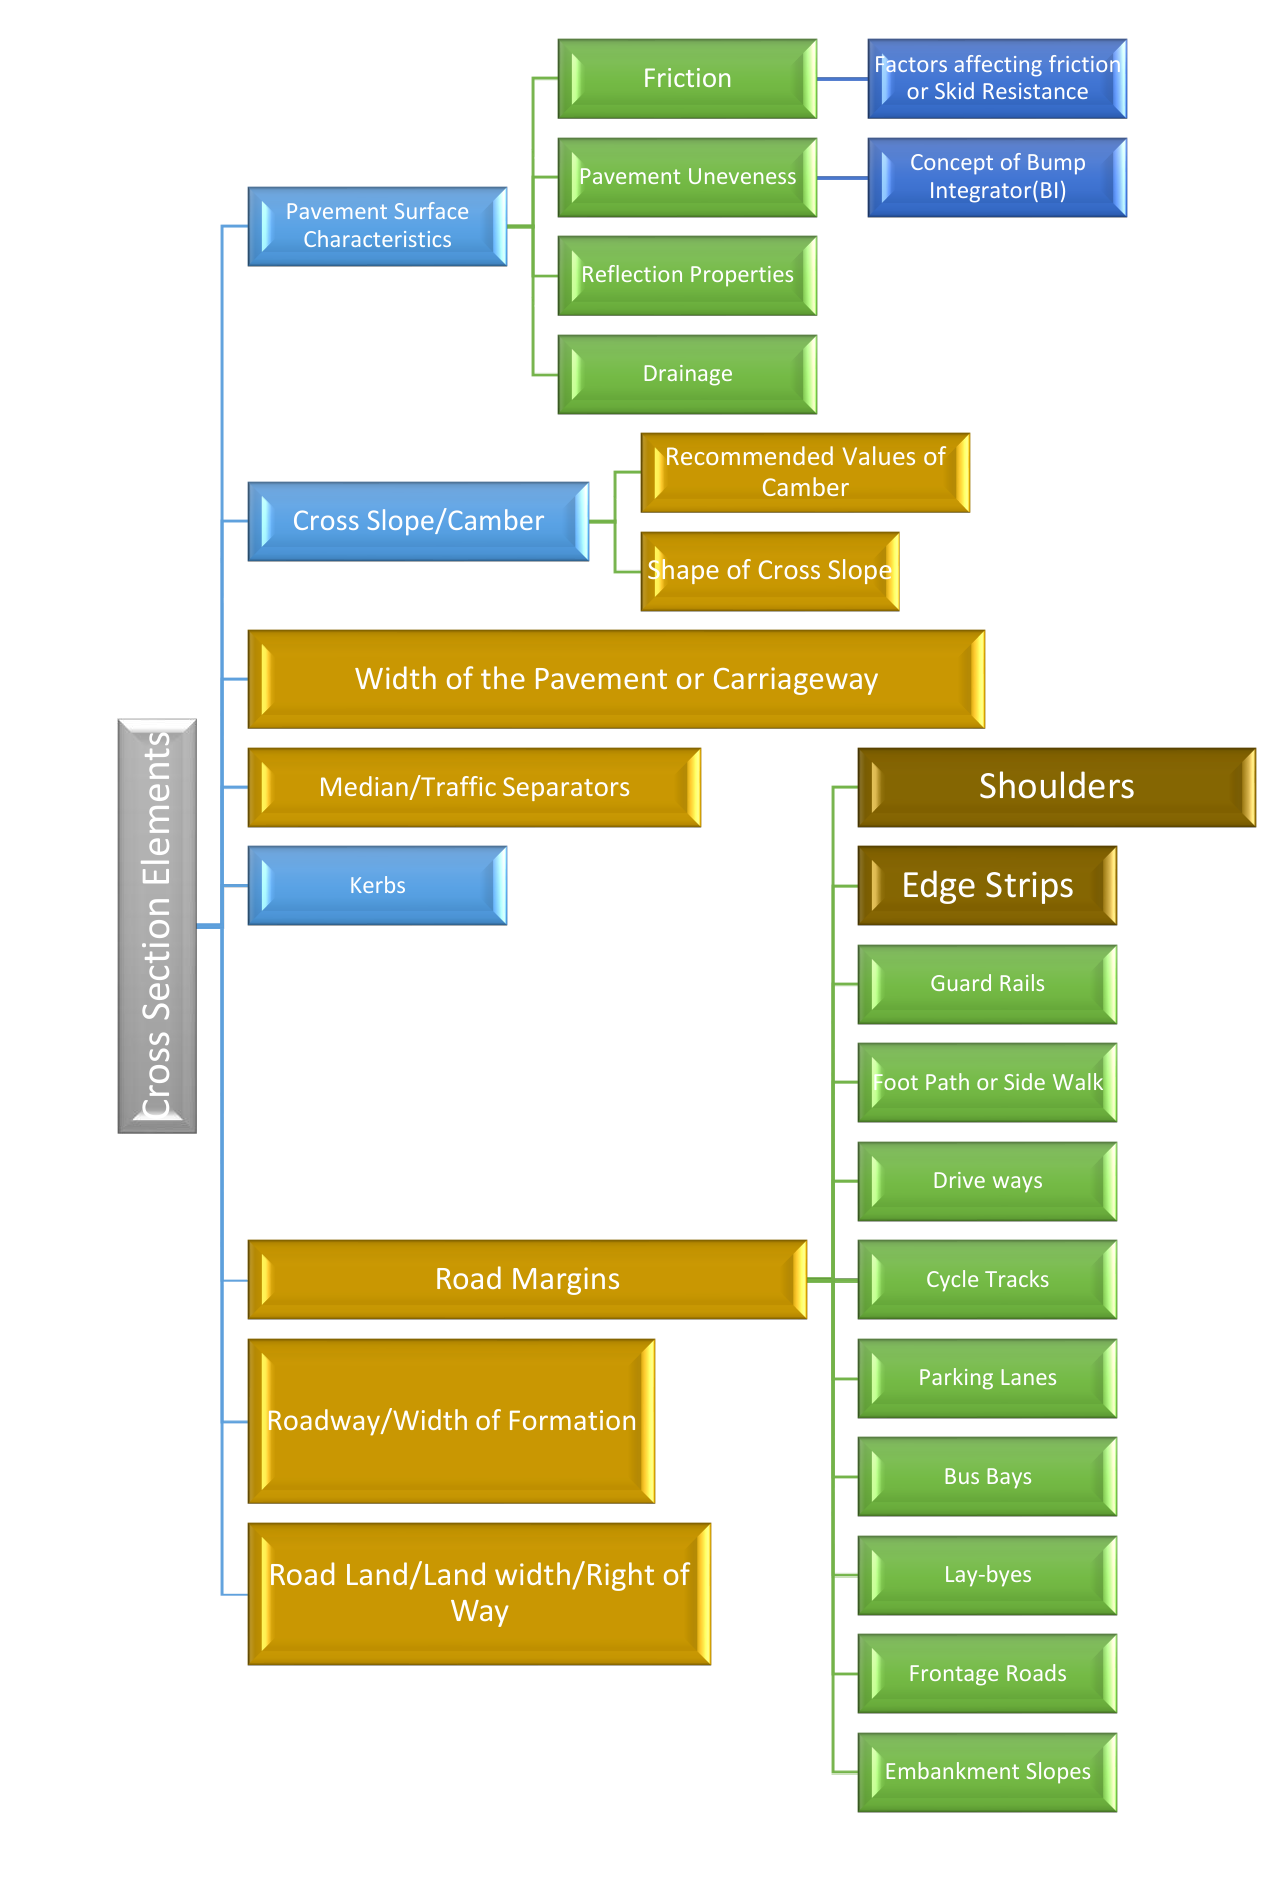
\includegraphics[width=0.85\textwidth]{fig_a3_cross_section_elements.png}
  \caption{Typical highway cross-section elements considered when identifying which elements apply to a tangent-section design (as reproduced in the original submission).}
  \label{fig:cross-section-elements}
\end{figure}

\begin{figure}[H]
  \centering
  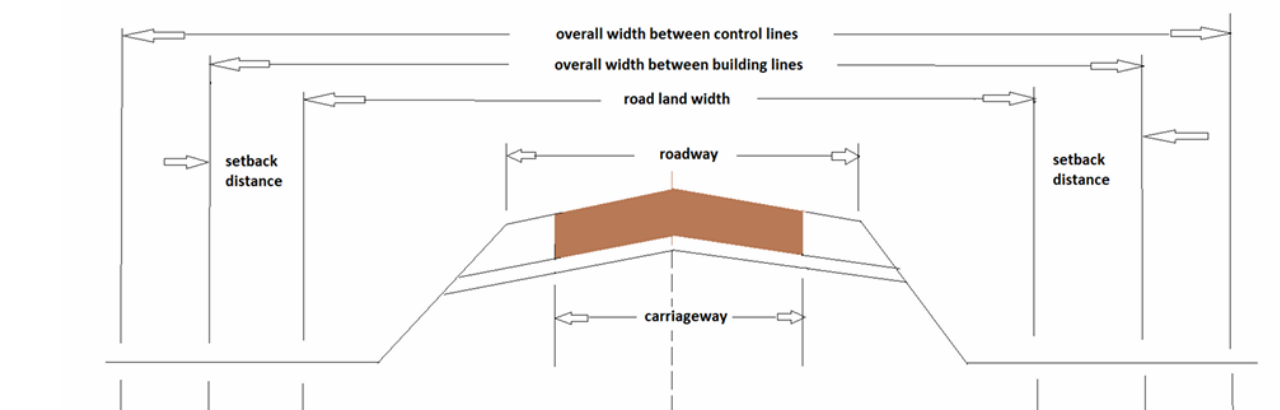
\includegraphics[width=0.8\textwidth]{fig_a3_typical_cross_section.png}
  \caption{Generic annotated highway cross-section showing roadway, carriageway, setback distance, building line, and control line terminology used in the design (as reproduced in the original submission).}
  \label{fig:typical-cross-section}
\end{figure}

\subsection{Design Considerations}
\begin{enumerate}
  \item \textbf{Location.} Open country in North-East India, with an annual rainfall of 200~cm.
  \item \textbf{Road classification.} Expressway (4-lane).
  \item \textbf{Pavement surface type.} IRC recommends a bituminous surface for high-speed roads.
  \item \textbf{Lane width.} Per IRC guidelines for expressways in plain and rolling terrain, the lane
  width is 3.75~m per lane; for a four-lane highway, total carriageway width $= 4 \times 3.5\,\text{m} =
  14\,\text{m}$.
  \item \textbf{Shoulder width.}
  \begin{itemize}
    \item Paved shoulder: minimum 3~m on both sides.
    \item Earthen shoulder: minimum 1.5~m on both sides.
    \item Total shoulder width $= 3 + 1.5 = 4.5\,\text{m}$.
  \end{itemize}
  \item \textbf{Median width.} A 10~m median is adopted (IRC/MoRTH minimum for expressways without a
  median barrier).
  \item \textbf{Service lane.} A service lane of 5~m is adopted.
  \item \textbf{Crossfall/camber.} For a bituminous surface in regions with heavy rainfall
  ($\geq 100$~cm), the camber is \textbf{2.5\%}.
  \item \textbf{Side slopes.} For expressways, embankment side slopes of 4H:1V or flatter are recommended
  for moderate-height embankments.
  \item \textbf{Right of way (RoW).} The RoW accommodates the roadway (carriageway, shoulders, median),
  side drains, service roads, and utilities. For a four-lane expressway in open country at a 100~km/h
  design speed, the RoW generally ranges up to \textbf{90~m} in plain/rolling terrain (per MoRTH
  guidelines for expressways).
  \item \textbf{Building and control lines.} Per MoRTH guidelines for expressways in plain/rolling
  terrain, the overall width between building lines is 110~m and the overall width between control lines
  is 130~m in open areas, with a 5~m distance between the building line and the RoW boundary in built-up
  areas.
\end{enumerate}

\begin{table}[H]
  \centering
  \caption{Summary of adopted cross-section parameters for the tangent section.}
  \begin{tabular}{@{}ll@{}}
    \toprule
    \textbf{Parameter} & \textbf{Adopted value} \\
    \midrule
    Carriageway width (4 lanes) & 14 m \\
    Paved shoulder (each side) & 3 m \\
    Earthen shoulder (each side) & 1.5 m \\
    Total shoulder width (each side) & 4.5 m \\
    Median width & 10 m \\
    Service lane & 5 m \\
    Camber (bituminous, rainfall $\geq$ 100 cm) & 2.5\% \\
    Embankment side slope & 4H:1V (or flatter) \\
    Right of way (plain/rolling terrain) & 90 m \\
    Width between building lines (open area) & 110 m \\
    Width between control lines (open area) & 130 m \\
    \bottomrule
  \end{tabular}
\end{table}

\textbf{Note on the graph-paper deliverable.} The question asked for the cross-section to be represented
on graph paper at a suitable horizontal and vertical scale. The submitted PDF for this assignment ends at
item~11 (Building and Control Lines) with the IRC/MoRTH reference tables reproduced above; it does not
contain a separate scaled, dimensioned cross-section drawing on graph paper beyond the generic annotated
diagram shown in Figure~\ref{fig:typical-cross-section}. This is reproduced here faithfully as submitted,
without inventing a graph-paper drawing that is not present in the original assignment.

\clearpage
\section{Assignment 4: Geometric Design and Safety Review of the H10 Intersection, IIT Bombay Campus}

\textbf{Group submission note:} This assignment was completed jointly with Karshan M.\ Kanjariya
(24D0322), Irfan Ali (24D0314), Menbere Aklilu (24D0315), and Fred Ssemwogerere (24D0326), as recorded on
the original submission's title page. The content below reproduces the submitted group report.

\textbf{Objective and scope.} The objective of this study is to conduct a geometric design and safety
evaluation of the H10 intersection within the IIT Bombay campus, grounded in the principles of
intersection design taught in CE~773. The evaluation is based on field observations, photographic
evidence, and intersection design guidelines, focusing on geometric elements such as sight distance,
alignment, pedestrian and cyclist integration, and signage placement.

\subsection{Location and Purpose of the Intersection}
The selected intersection is located near Hostel 10 (H10) on the IIT Bombay campus, connecting the H14
hostel road, the H12 hostel approach, and a minor arm leading toward CCD and the KV School. It
facilitates movement for hostel residents (pedestrians and cyclists), institutional traffic (autos,
service vehicles), and access to key campus facilities (IDC, Hostels 10, 12, 14), experiencing moderate
daily traffic as a T-intersection with a mixed user group.

\begin{figure}[H]
  \centering
  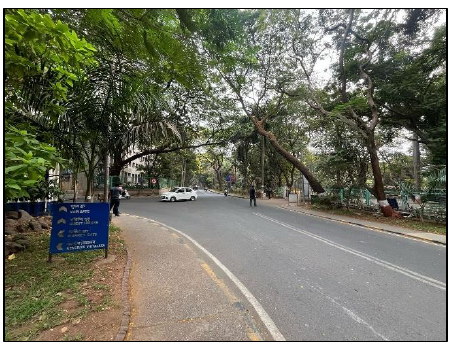
\includegraphics[width=0.7\textwidth]{fig_a4_site_photo_h12.png}
  \caption{View from the H12 side toward the intersection, with visible signage and road curvature (Fig.\ 1 of the original submission).}
\end{figure}

\begin{figure}[H]
  \centering
  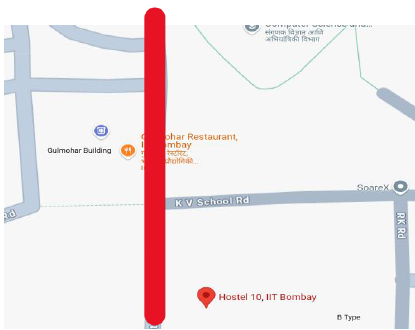
\includegraphics[width=0.65\textwidth]{fig_a4_map_view.png}
  \caption{Google Maps aerial view of Hostel 10 and the surrounding intersection (Fig.\ 2 of the original submission).}
\end{figure}

\subsection{Existing Layout and Traffic Movement}
\begin{itemize}
  \item \textbf{Intersection type:} 3-legged (T-intersection), near H10 and H12 hostels.
  \item \textbf{Traffic control features:} no yield or stop sign is provided; the intersection operates
  in an uncontrolled condition, relying on driver judgment and road-user negotiation.
  \item \textbf{Lane and movement characteristics:} each leg consists of two lanes with two-way traffic
  permitted; all turning movements are allowed, including right turns from the minor leg (H12) onto the
  major road and left turns into/from all approaches.
  \item \textbf{Traffic composition:} a heterogeneous mix of passenger vehicles (cars, two-wheelers,
  autorickshaws), non-motorized users (pedestrians and cyclists), and service/delivery vehicles
  (including light and heavy commercial vehicles accessing the SAC and hostels).
  \item \textbf{Geometric challenges from movement:} the absence of channelization and traffic control
  creates crossing conflicts between right-turning vehicles and oncoming traffic, merging/diverging
  conflicts at the T-junction without geometric separation, and pedestrian--vehicle confusion due to the
  lack of crosswalks and refuge islands.
\end{itemize}

\subsection{Conflict Point Analysis}
Based on the turning and through-movement possibilities at this three-legged unsignalized intersection,
the following conflict points were identified.

\begin{table}[H]
  \centering
  \caption{Conflict point count at the H10 intersection.}
  \begin{tabular}{@{}lr@{}}
    \toprule
    \textbf{Conflict type} & \textbf{Count} \\
    \midrule
    Crossing conflicts  & 3 \\
    Merging conflicts   & 4 \\
    Diverging conflicts & 4 \\
    \textbf{Total conflicts} & \textbf{11} \\
    \bottomrule
  \end{tabular}
\end{table}

\begin{figure}[H]
  \centering
  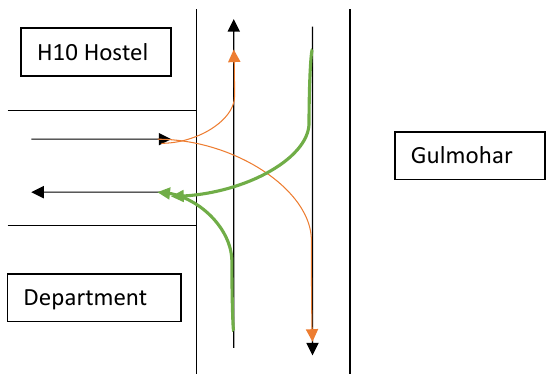
\includegraphics[width=0.6\textwidth]{fig_a4_conflict_diagram.png}
  \caption{Schematic of traffic movements at the H10 intersection (H10 Hostel, Department, and Gulmohar arms), used to enumerate crossing, merging, and diverging conflict points.}
\end{figure}

\textbf{Observation of conflict risk -- obstructed sight triangle.} Right-turning vehicles from the H12
approach face visibility issues due to vegetation or parked vehicles, increasing the likelihood of
side-impact conflicts at crossing points.

\begin{figure}[H]
  \centering
  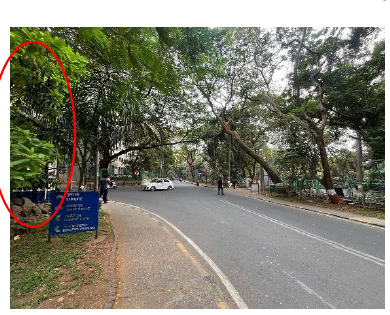
\includegraphics[width=0.55\textwidth]{fig_a4_block_visibility.png}
  \caption{Block Visibility: vegetation obstructing the sight triangle at the H12 approach (Fig.\ 3 of the original submission).}
\end{figure}

\textbf{No pedestrian crossings.} Without marked crossings or refuge islands, pedestrians cross
informally, creating uncontrolled pedestrian-vehicle conflict zones that overlap with vehicle paths.
\textbf{Lack of regulatory signs or markings.} The absence of Stop or Give Way signs and markings means
drivers must guess priority, leading to unregulated merging and diverging behavior, especially during
peak hostel hours.

\begin{figure}[H]
  \centering
  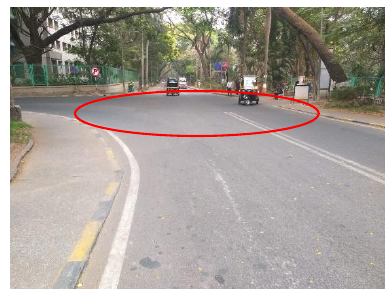
\includegraphics[width=0.55\textwidth]{fig_a4_no_zebra_crossing.png}
  \caption{No Zebra-Crossing near intersection (Fig.\ 4 of the original submission).}
\end{figure}

\subsection{Skew Angle and Intersection Geometry}
Based on the layout and road alignment visible in the field map and physical inspection, the angle of
intersection formed at the H10 intersection is estimated to be approximately \textbf{85\textdegree\ to
90\textdegree}. The recommended angle for direct crossings is 75\textdegree--105\textdegree\ per standard
design guidelines; the H10 intersection falls within this range and is therefore classified as a
``Direct'' intersection geometry.

\subsection{Sight Triangle Evaluation}
\textbf{Intersection control type: Case A -- No Control.} There are no stop signs, yield signs, or
signals on any approach; drivers must rely entirely on visual judgment to identify gaps and cross
conflicting traffic streams.

\subsection{Problem Identification}
\begin{enumerate}
  \item \textbf{Lack of dedicated space for non-motorized users.} No cycle lanes or shared
  pedestrian-bicycle pathways, leading to conflicts between vulnerable users and motorized vehicles.
  \item \textbf{Inadequate and obstructed traffic signage.} Traffic signs are either too small, poorly
  placed, or hidden by vegetation, reducing their visibility and effectiveness.
  \item \textbf{Unclear right-of-way due to missing regulatory elements.} No Stop or Give Way signs or
  pavement markings, resulting in driver confusion and unregulated movement.
  \item \textbf{Non-standard and unsafe pedestrian infrastructure.} Uneven kerbs at bell mouths,
  non-uniform walkway heights, and speed breakers and footpaths at the same level.
\end{enumerate}

\begin{figure}[H]
  \centering
  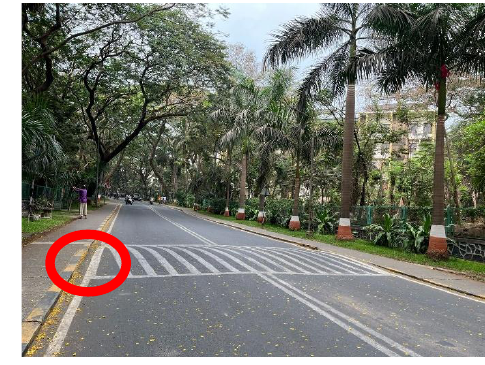
\includegraphics[width=0.55\textwidth]{fig_a4_speed_breaker_footpath.png}
  \caption{Same level of speed breaker and footpath (Fig.\ 5 of the original submission).}
\end{figure}

\begin{figure}[H]
  \centering
  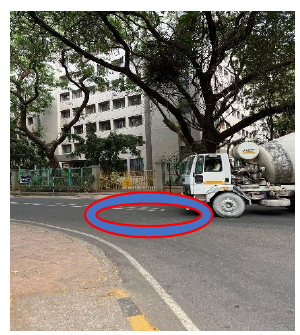
\includegraphics[width=0.5\textwidth]{fig_a4_missing_pavement_marking.png}
  \caption{Missing Pavement Marking: faded or missing pavement markings reduce lane definition and visual guidance, especially under low-light or wet conditions (Fig.\ 6 of the original submission).}
\end{figure}

\begin{enumerate}
  \setcounter{enumi}{4}
  \item \textbf{Sunken or damaged kerbs.}
\end{enumerate}

\begin{figure}[H]
  \centering
  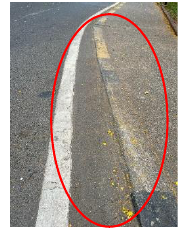
\includegraphics[width=0.35\textwidth]{fig_a4_damaged_kerb.png}
  \caption{Damaged Kerb (Fig.\ 7 of the original submission).}
\end{figure}

\subsection{Geometric Design Evaluation}
\begin{table}[H]
  \centering
  \caption{Geometric design evaluation ratings.}
  \begin{tabular}{@{}ll@{}}
    \toprule
    \textbf{Category} & \textbf{Rating} \\
    \midrule
    Uniformity            & Needs Improvement \\
    Conflict Minimization & Needs Improvement \\
    Safety                & Poor \\
    Alignment \& Profile  & Acceptable \\
    \bottomrule
  \end{tabular}
\end{table}

\subsection{Conclusion}
While the intersection geometry (angle and profile) is acceptable, the overall intersection design does
not align well with core design principles: the lack of regulatory signage and markings undermines
simplicity and uniformity; high conflict points and unmarked user paths raise safety concerns; and the
absence of pedestrian and cyclist facilities makes the intersection non-inclusive. This makes a strong
case for geometric redesign, particularly through channelization, visibility clearance, signage and
markings, and dedicated paths for non-motorized transport (NMT).

\subsection{Proposed Design Improvements}

\textbf{A. Non-motorized user facilities.}
\begin{enumerate}
  \item Dedicated cycle lanes / shared pedestrian-cyclist pathways along intersection arms, to reduce
  lateral conflicts between vulnerable users and motorized vehicles.
  \item Marked pedestrian crosswalks (zebra crossings) on all legs to channel pedestrian movement.
  \item Uniform pedestrian walkway height across approaches, to eliminate tripping risks.
  \item Level kerbs, with standardized curb heights near turning zones for safer pedestrian crossing
  transitions.
\end{enumerate}

\textbf{B. Speed control and driver behavior management.}
\begin{enumerate}
  \setcounter{enumi}{4}
  \item Speed breakers / rumble strips on all approaches at appropriate distances, to reduce speed and
  improve driver attention.
  \item Rectify the oversized speed hump on the H12 arm, adjusting its height so the walkway remains
  elevated and the hump provides only mild deceleration.
  \item Post speed-limit signboards (e.g., 25--30 km/h) using standard campus signage.
\end{enumerate}

\textbf{C. Signage, markings, and priority control.}
\begin{enumerate}
  \setcounter{enumi}{7}
  \item Install regulatory signs (STOP / GIVE WAY) on the H12 approach and other minor arms to assign
  clear right-of-way priority.
  \item Replace obscured or small traffic signs with more prominent retro-reflective signs, placed at
  standard eye level and cleared of vegetation.
\end{enumerate}

\textbf{D. Visibility and sight triangle enhancements.}
\begin{enumerate}
  \setcounter{enumi}{11}
  \item Clear the sight triangle on the H12 arm by removing vegetation and visual obstructions within
  25--30~m of the driver's decision point on the minor arm.
\end{enumerate}

\textbf{E. Geometric redesign suggestions.}
\begin{enumerate}
  \setcounter{enumi}{12}
  \item Repair or replace sunken median kerbs, using raised medians or plastic channelizers to clearly
  separate turning traffic and discourage corner-cutting.
  \item Close the Canara Bank driveway entry, blocking vehicular entry from the bank side near the
  junction, which currently introduces unexpected diverging paths and increases merge conflicts.
\end{enumerate}

\begin{table}[H]
  \centering
  \caption{Summary of proposed improvement categories and key actions.}
  \begin{tabular}{@{}ll@{}}
    \toprule
    \textbf{Category} & \textbf{Key action} \\
    \midrule
    Pedestrian/cyclist safety & Crosswalks, kerb levelling, shared pathways \\
    Speed control             & Rumble strips, proper hump design, signs \\
    Traffic control           & STOP/GIVE WAY signs and markings \\
    Visibility                & Sight-triangle clearance, sign upgrades \\
    Geometric enhancements    & Kerb repairs, channelization, driveway closure \\
    \bottomrule
  \end{tabular}
\end{table}

\end{document}
